

\section{Case Study: Git}
We started with a legacy Git model, and aimed to validate and improve it.
Our goal was to create a testbench that implements model validation through test case generation applied to this git model so that we could test git itself, and improve the model.
Our testbench uses the Git Alloy model and the Alloy API to implement model validation through test case generation



\section{ValidAlloy Features}
Our Testbench is capable of:
\begin{itemize}
\item Creating a git repo from the modelled instance;
\item Associating any git modelled command with actual command;
\item Comparing the modelled version with the git command;
\item Generic configuration file;
\item Handles git errors.
\end{itemize}


It is configured through a configuration file that lets you make those associations and other important configurations.
The tool also leaves the Alloy instance xml in the git repo that was generated from it, and saves extensive logs, so that the user is capable of fully analyse the results of the testbench.
It distinguishes between an error occurring in an operation and an operation returning different results than those expected.This is important to know what change in the model (errors means the current pre-conditions are too weak, and different results means wrong post-conditions), unless it is an actual git bug.

\begin{figure}[H]
\centering
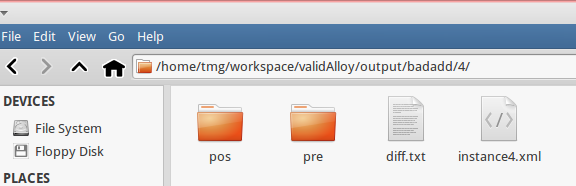
\includegraphics[width=\textwidth]{images/INSIDE.png}
\caption{Pre and Pos state}
\end{figure}

\section{Implementation Details}

We decided to implement ValidAlloy with Java7 mainly because we are using an Alloy model, and Alloy has a Java API that we find very helpful to make the process automatic.
Our tool depends on the Git Alloy model, this implies that if you change some parts of the model, you might have to change the testbench.(The structural part of the model(sigs and facts) must remain the same for the testbench to work but predicates can be changed without need to change the testbench)
It only supports predicates written on that model.
It requires as input a configuration file.

\begin{figure}[H]
\centering
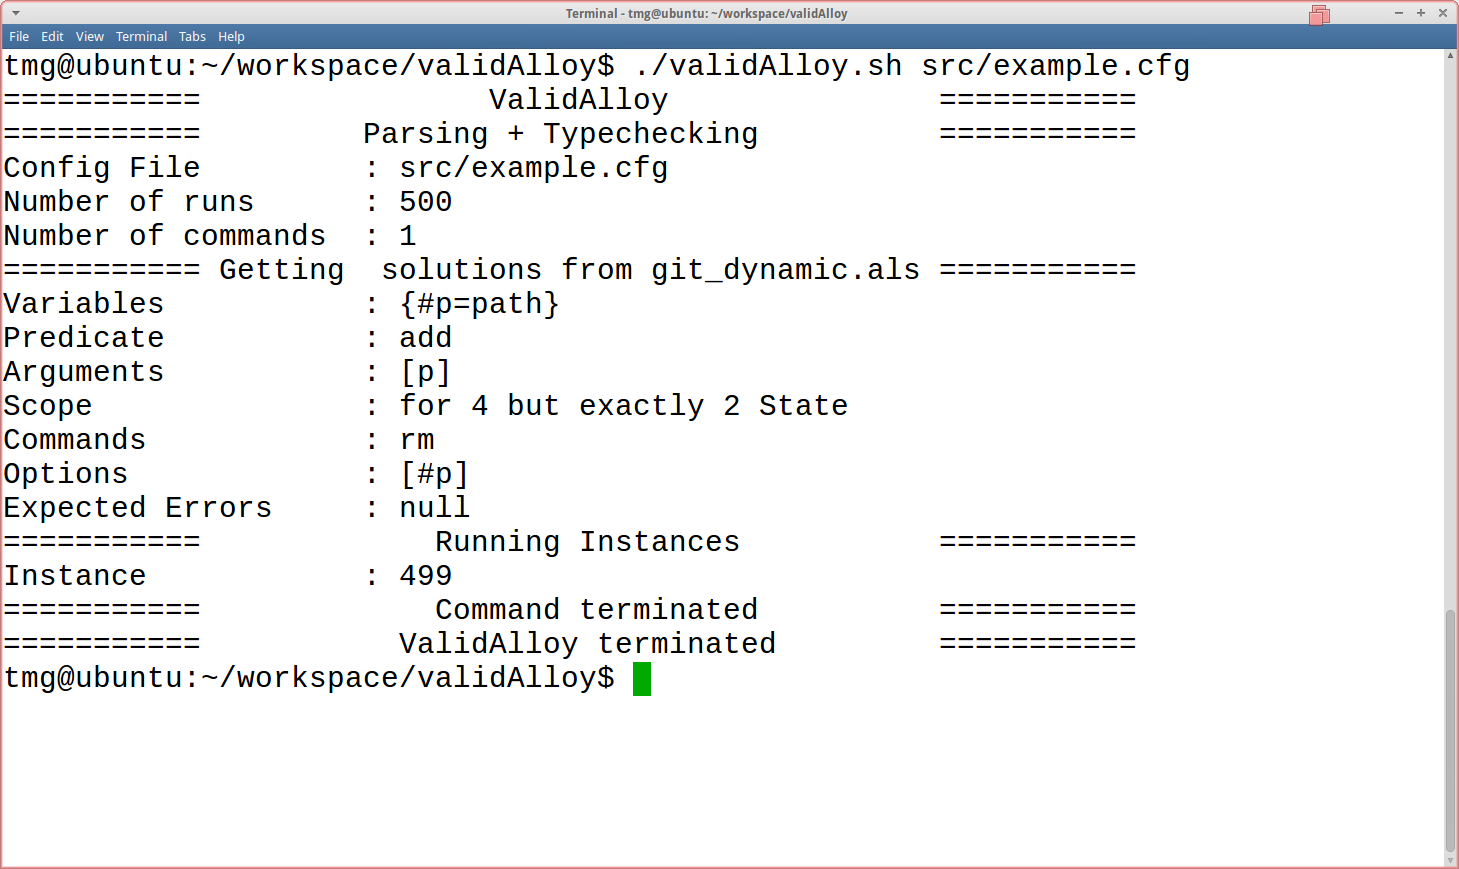
\includegraphics[width=\textwidth]{images/SHELL.png}
\caption{A run of validalloy}
\end{figure}

\section{How it works}

A configuration file is passed as input to the testbench, in this file should the the associations between the model predicates and the actual git commands, it should also be present the number of test runs.
Through the Alloy API, the testbench generates the model instances, for each instance it is created two different folders, one with the a git repository to be used to run the  command, the other contains the git repository that is expected as result.
We use Git plumbing commands to generate the git objects.
After everything need is created, the git command runs, if the commands reports an error, it is saved in an error file, otherwise the testbench will compare both folders and create a file with all differences listed if they exist.
By default our testbench deletes successfully runs(runs with no errors, and no differences between the expected result and the actual result).

\begin{figure}[H]
\centering
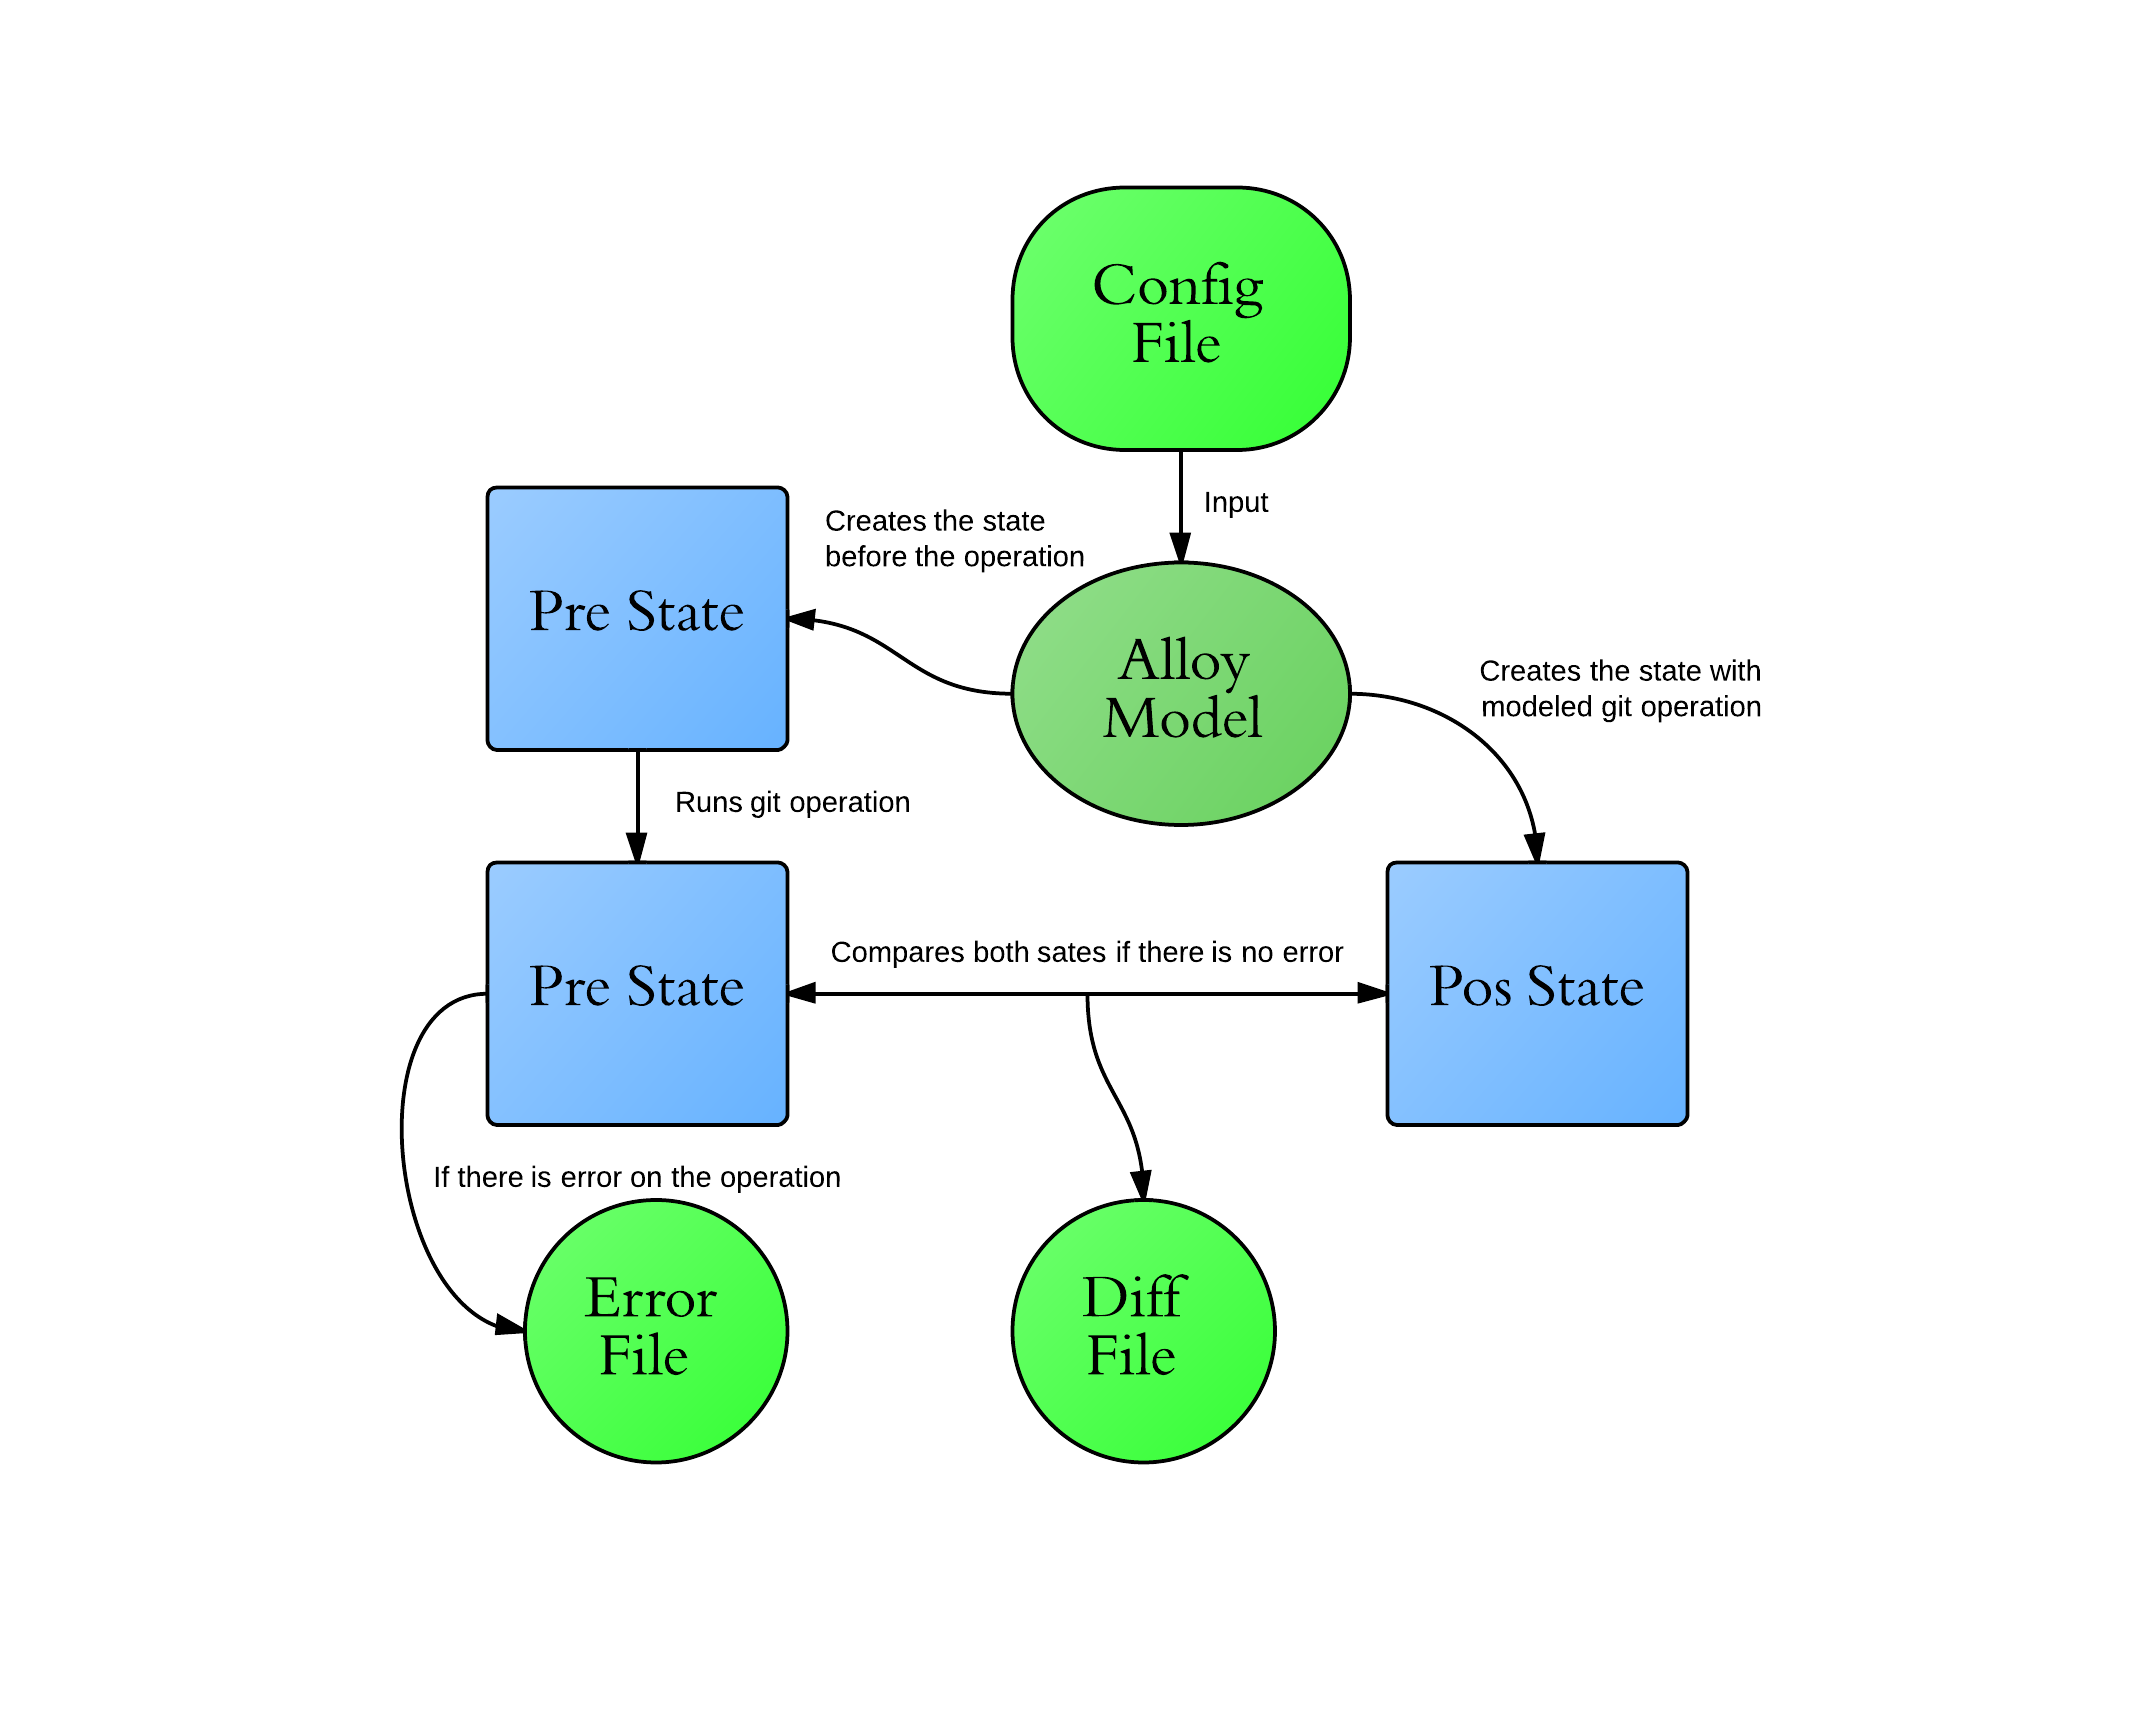
\includegraphics[width=\textwidth]{images/workflow.png}
\caption{How it works}
\end{figure}

\begin{figure}[H]
\centering
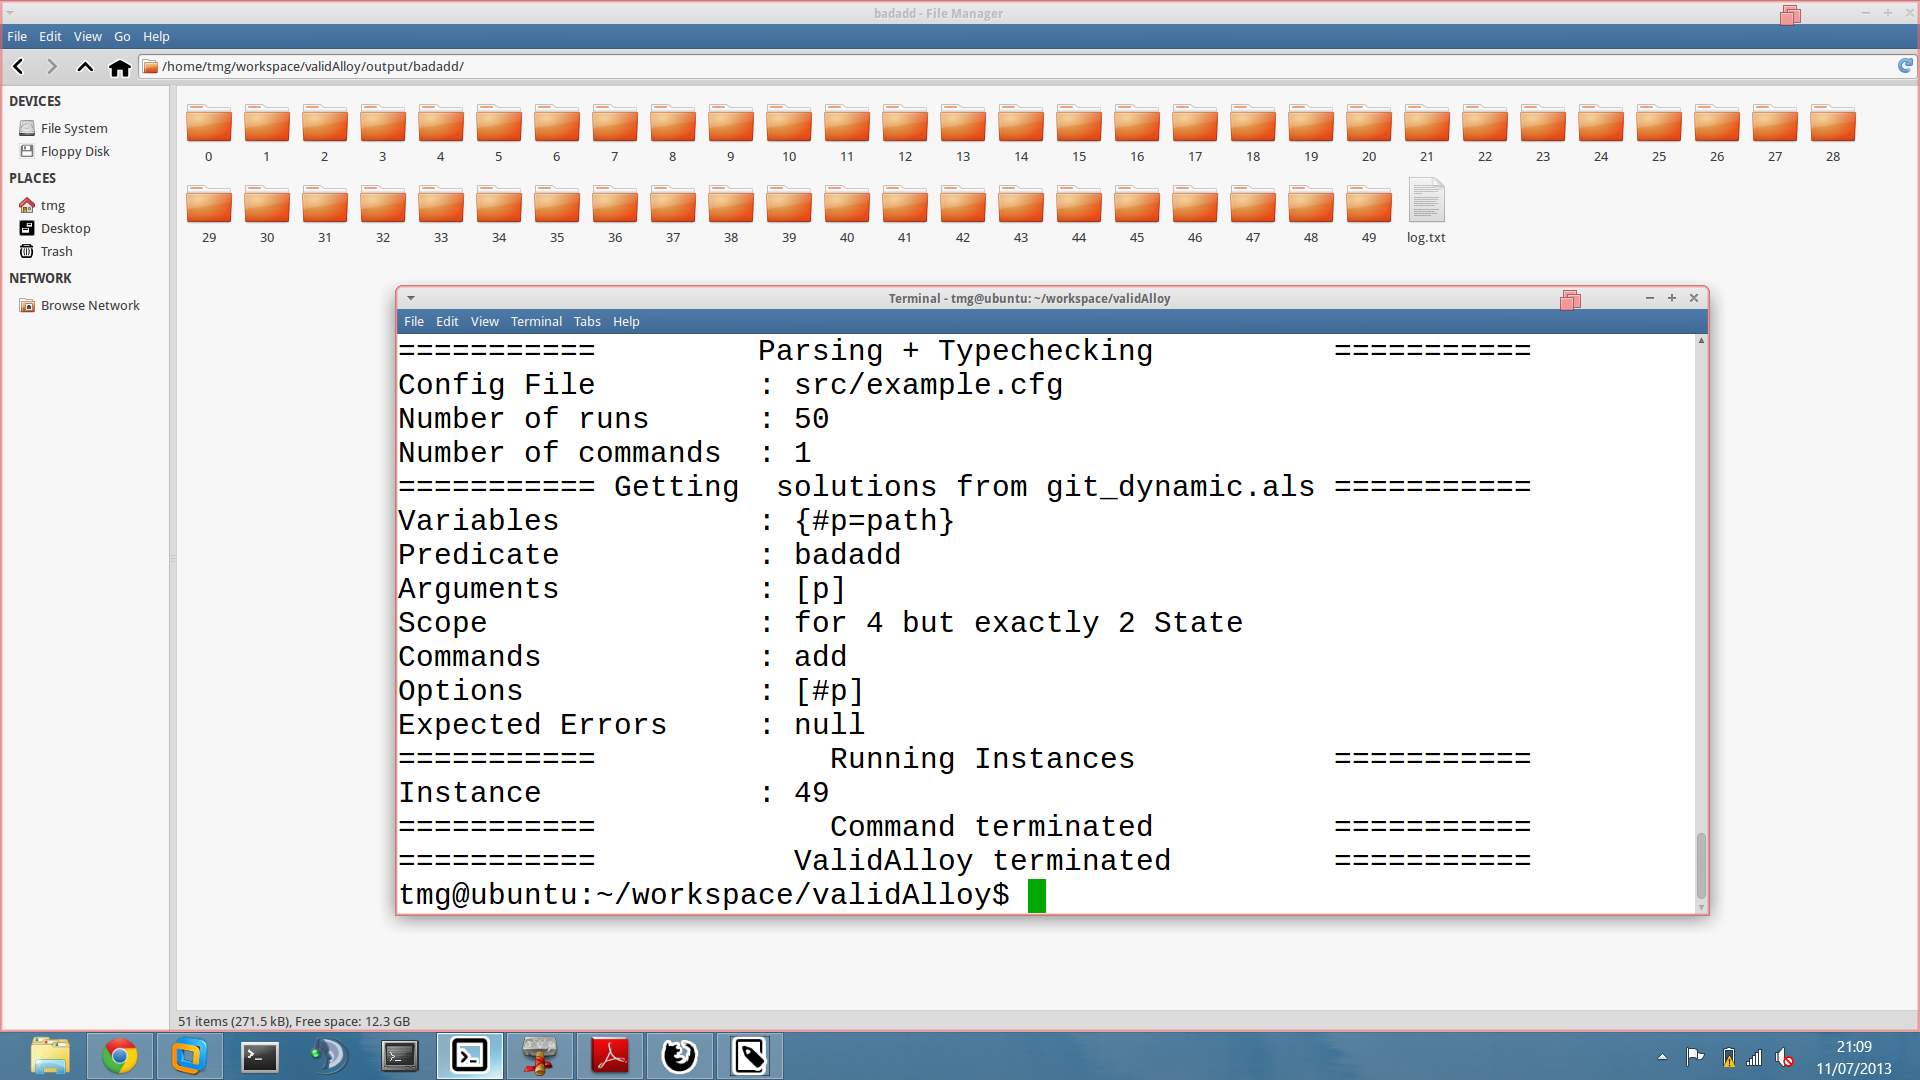
\includegraphics[width=\textwidth]{images/PASTAS.png}
\caption{A run of validalloy with bad modelled add, showing folders with differences}
\end{figure}

\subsection{Alloy API}
Our testbench relies a lot on the Alloy API, every alloy run is executed through it, and it is used to iterate the result models so that we could create the git repositories.
We use the API to parse the model from the file, then we use the the method CompUtil.parseOneExpression\_fromString to create the expressions that we needed to use, but we still had to build some expressions manually, this was because we couldn't get the instance atoms with this method, so after we evaluate we had to look up on an previously created map, to get the corresponding expression to an atom.

\subsection{Git plumbing commands}
To create the git objects, we used several git low level\cite{gitpro}\cite{git_man} commands those where:
\begin{itemize}
\item git hash-object : creates the blobs;
\item git mktree : creates the git filesystem tree;
\item git commit-tree : creates the git commit tree;
\item git symbolic-ref HEAD : sets the HEAD to a ref;
\item git update-ref : creates the refs;
\item git update-index : creates the index file.
\end{itemize}
\newpage
\subsection{Unix Diff}
The Unix diff is the key to our repository comparation, not only because it precisely reports differences in files, but also because if you use the -r flag it will compare everything that exist on the given folders.
Because we relay on diff, our testbench will only work on Unix systems.

\begin{figure}[H]
\centering
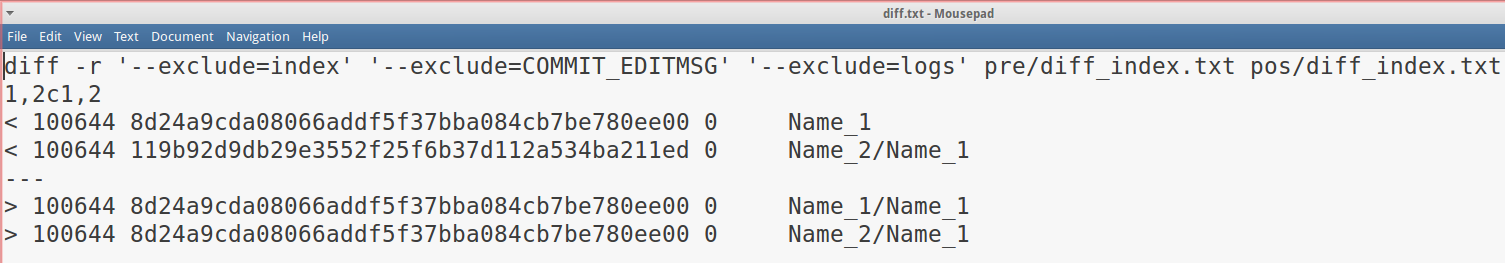
\includegraphics[width=\textwidth]{images/DIFS.png}
\caption{Example diff file}
\end{figure}

\subsection{Configuration File}

To generate the parser to parse our config file, we used Another Tool For Language Recognition \cite{antlr}. 

Our language is very simple, you define a list of commands, where each command has a a list of variables, the predicate that must be run, its scope, the associated git command and its parameters and a list of expected errors, finally you have the number of iterations that validalloy must run. For a formal description of the grammar go to appendix A. Bellow follows a config file example:

\begin{lstlisting}[caption=Config file example]
#p : path
pred rmNOP[#p]
scope for 4 but exactly 2 State
cmd git rm #p
errors ("has changes staged in the index")  

runs 100
\end{lstlisting}

\subsection{Logs}

Early during the development of our testbench, we realized that we needed to record our operations and the output of the the git commands, we had to implement logs.


We were concerned that due to the big amount of io operations that our testbench does, adding a powerful but complex log system(like log4j) would stress the testbench even more, so we choose java tinylog, mainly because it is fast, has a small memory footprint and supports writing threads.

Our logs support different levels:
\begin{itemize}
\item TRACE: Result of a successfully operation;
\item ERROR: When a operation returns an error;
\item INFO: Normal behaviour of the testbench.
\end{itemize}
When a predicate is run, all the logs of the testbench are written to that predicate output folder in a file named logs.txt.
\newpage
\section{Problems encountered}

During the development of ValidAlloy we had some problems to related to the approach we were using that we had resolve:
\begin{itemize}
\item Timestamps in commit objects: We resolved this problem, by fixing the same time-stamp in all commit objects;
\item Index is binary file and difficult to compare: Instead of comparing the index file, we ignore it, and compare the output from git ls-files -staged instead, this command already gives us everything we modelled about the index.
\item Errors that are expected while running the git operations: We added to the config file a list of expected errors;
\item Git doesn't report some "errors" as errors, but to standard input: We could not find a solution to this problem, but you can manually check the logs, and see if the output from the operation was actually an error.
\end{itemize}
